\documentclass{beamer}

\setlength{\parskip}{1em}

\title{GRAH-BERT Review}
\subtitle{Alex To}

%\usetheme{lucid}
\begin{document}
	\frame {
		\titlepage
	}

	\frame{
		\frametitle{Agenda}
		
		\begin{itemize}
			\item Introduction
			\item Linkless subgraph Batching	
			\item Node input vector embeddings
			\begin{itemize}
				\item Raw feature vector embedding
				\item Weisfeiler Lehman absolute role embedding
				\item Intimacy based relative positional embedding
				\item Hop based relative distance embedding 
			\end{itemize}
			\item Embeddings aggregations
			\item Graph Transformer based encoder
			\item GRAPH-BERT learning
			\begin{itemize}
				\item Pre-training
			\end{itemize}
		\end{itemize}
	}

	\frame {
		\frametitle{Introduction}
		\begin{itemize}
			\item A graph neural network model
			\item Based on attention mechanism
			\item Train with sampled linkless subgraphs
		\end{itemize}
		\begin{figure}[htb]
			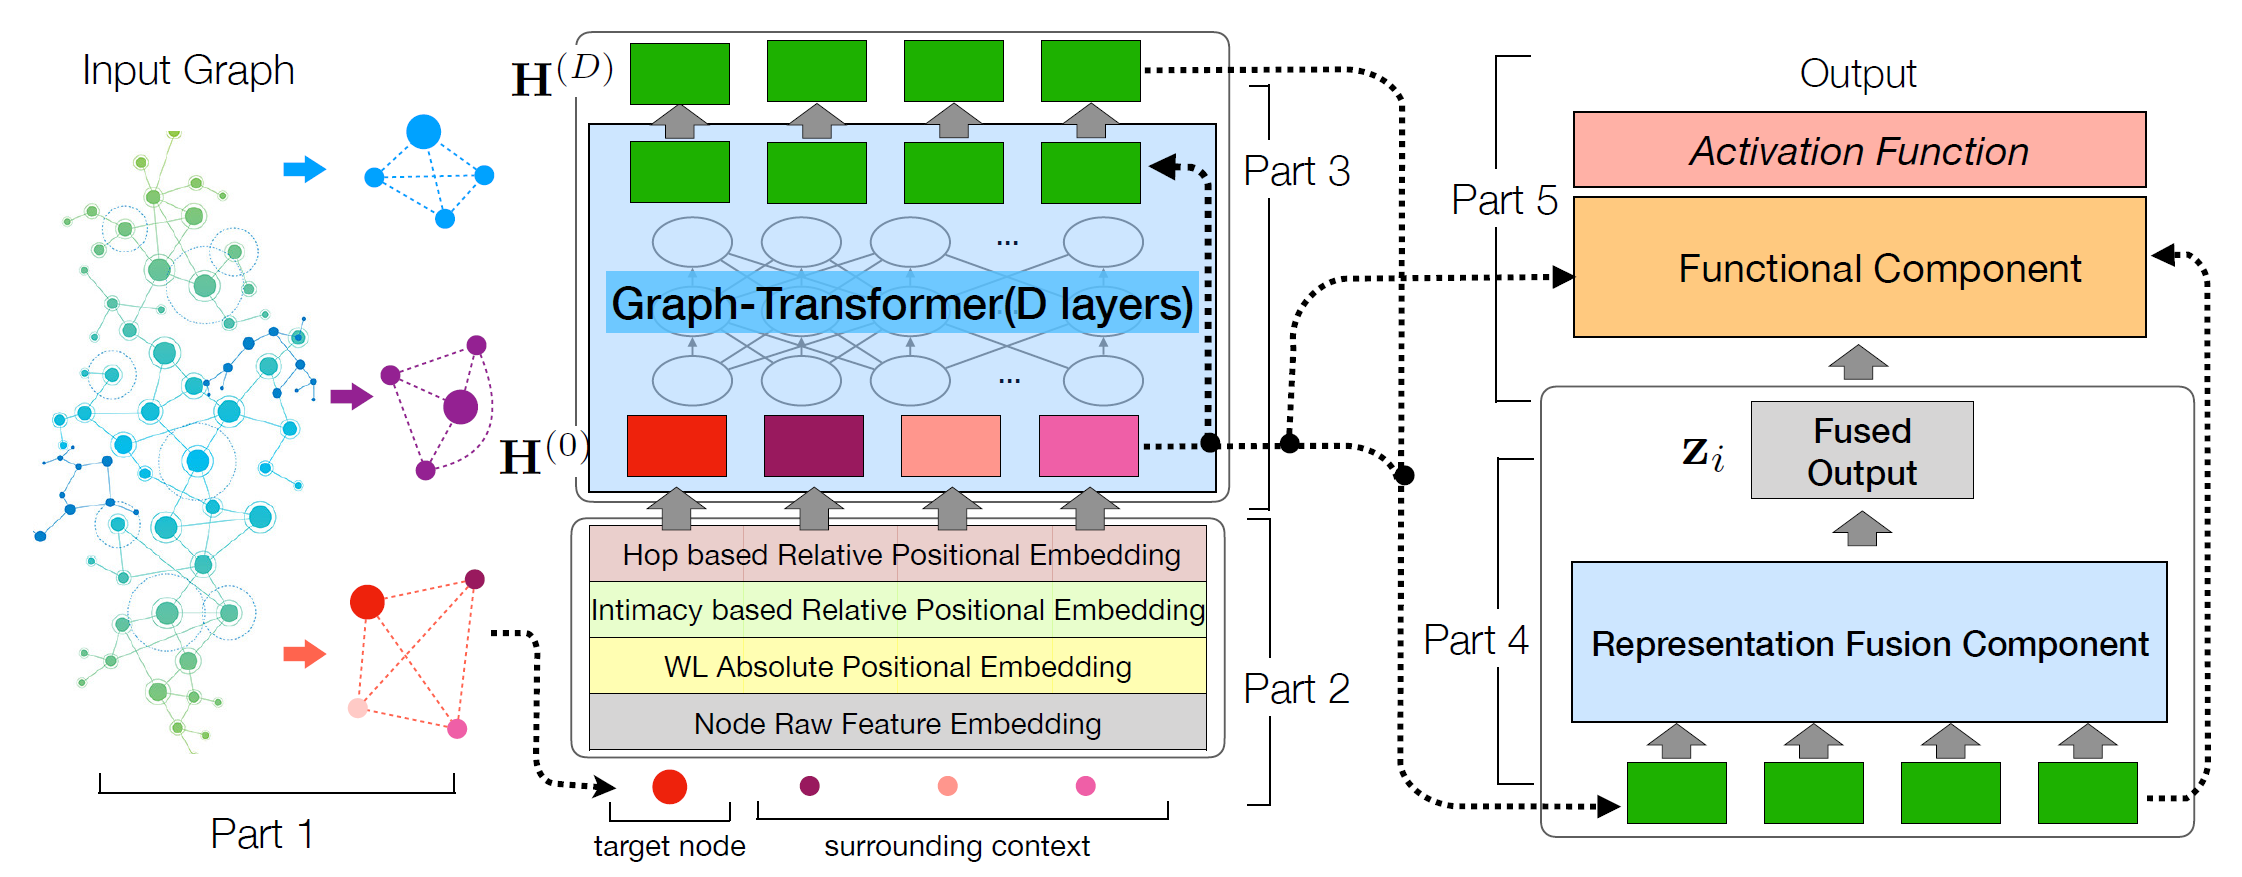
\includegraphics[width=1.0\textwidth]{figures/graph-bert-overview}
			\caption{GRAPH-BERT architecture}
		\end{figure}
	}

	\frame{ 
		\frametitle{Linkless subgraph batching}
		Given a graph $G(V,E)$ how to generate sub graph batches?
		
		\begin{itemize}
			\item Calculate an intimacy score matrix $S$
			\[
				S = \alpha \cdot (I - (1 - \alpha) \cdot \bar{A})^{-1}
			\]
			where 
			\[
				\bar{A} = AD^{-1}
			\]
			$A$: adjacency matrix	
			
			$D$: neighbor count diagonal matrix
		
			\item Based on $S$, for a target node $v_i$, find top $k$ "intimate" nodes of $v_i$ with $k$ largest $S(v_i, v_j)$ score.
		\end{itemize}			
	}
	
	\frame {
		\frametitle{Linkless subgraph batching (cont)}
		\begin{minipage}{\textwidth}
			\begin{columns}[T,onlytextwidth]
				\begin{column}{.4\textwidth}
					\begin{figure}
						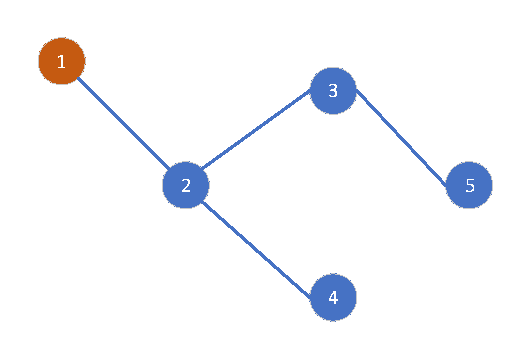
\includegraphics[width=0.9\textwidth]{figures/example-network}
					\end{figure}
				\end{column}
				\begin{column}{.45\textwidth}
					$A = \begin{bmatrix}
					0 & 1 & 0 & 0 & 0 \\
					1 & 0 & 1 & 1 & 0 \\
					0 & 1 & 0 & 0 & 1 \\
					0 & 1 & 0 & 0 & 0 \\
					0 & 0 & 1 & 0 & 0
					\end{bmatrix}$
				\end{column}
			\end{columns}
		\end{minipage}		
	    \begin{onlyenv}<2>
			\begin{minipage}{\textwidth}
				\begin{columns}[T,onlytextwidth]
					\begin{column}{.5\textwidth}
						$D = \begin{bmatrix}
						1 & 0 & 0 & 0 & 0 \\
						0 & 3 & 0 & 0 & 0 \\
						0 & 0 & 2 & 0 & 0 \\
						0 & 0 & 0 & 1 & 0 \\
						0 & 0 & 0 & 0 & 1
						\end{bmatrix}$
					\end{column}
					\begin{column}{.5\textwidth}
						$D^{-1} = \begin{bmatrix}
						1 & 0 & 0 & 0 & 0 \\
						0 & 1/3 & 0 & 0 & 0 \\
						0 & 0 & 1/2 & 0 & 0 \\
						0 & 0 & 0 & 1 & 0 \\
						0 & 0 & 0 & 0 & 1
						\end{bmatrix}$
					\end{column}
				\end{columns}
			\end{minipage}	
		\end{onlyenv}
	}

	\frame {
		\frametitle{Linkless subgraph batching (cont)}
		\begin{minipage}{\textwidth}
			$AD^{-1} = \begin{bmatrix}
			0 & 1/3 & 0 & 0 & 0 \\
			1 & 0 & 1/2 & 1 & 0 \\
			0 & 1/3 & 0 & 0 & 1 \\
			0 & 1/3 & 0 & 0 & 0 \\
			0 & 0 & 1/2 & 0 & 0
			\end{bmatrix}$	
		\end{minipage}
		

		
		\begin{minipage}{\textwidth}
			$S = \begin{bmatrix}
			0.259 & 0.128 & 0.085 & 0.109 & 0.072 \\
			0.386 & 0.454 & 0.302 & 0.386 & 0.257 \\
			0.171 & 0.201 & 0.369 & 0.171 & 0.313 \\
			0.109 & 0.128 & 0.085 & 0.259 & 0.072 \\
			0.072 & 0.085 & 0.156 & 0.072 & 0.283 
			\end{bmatrix}$
		\end{minipage}	
	
		For a target node $v_i$, take $k$ entries in $sorted(S(i,:))$, no links (hence, linkless subgraph)
	}

	\frame {
		\frametitle{Node input vector embeddings}
		\begin{figure}
			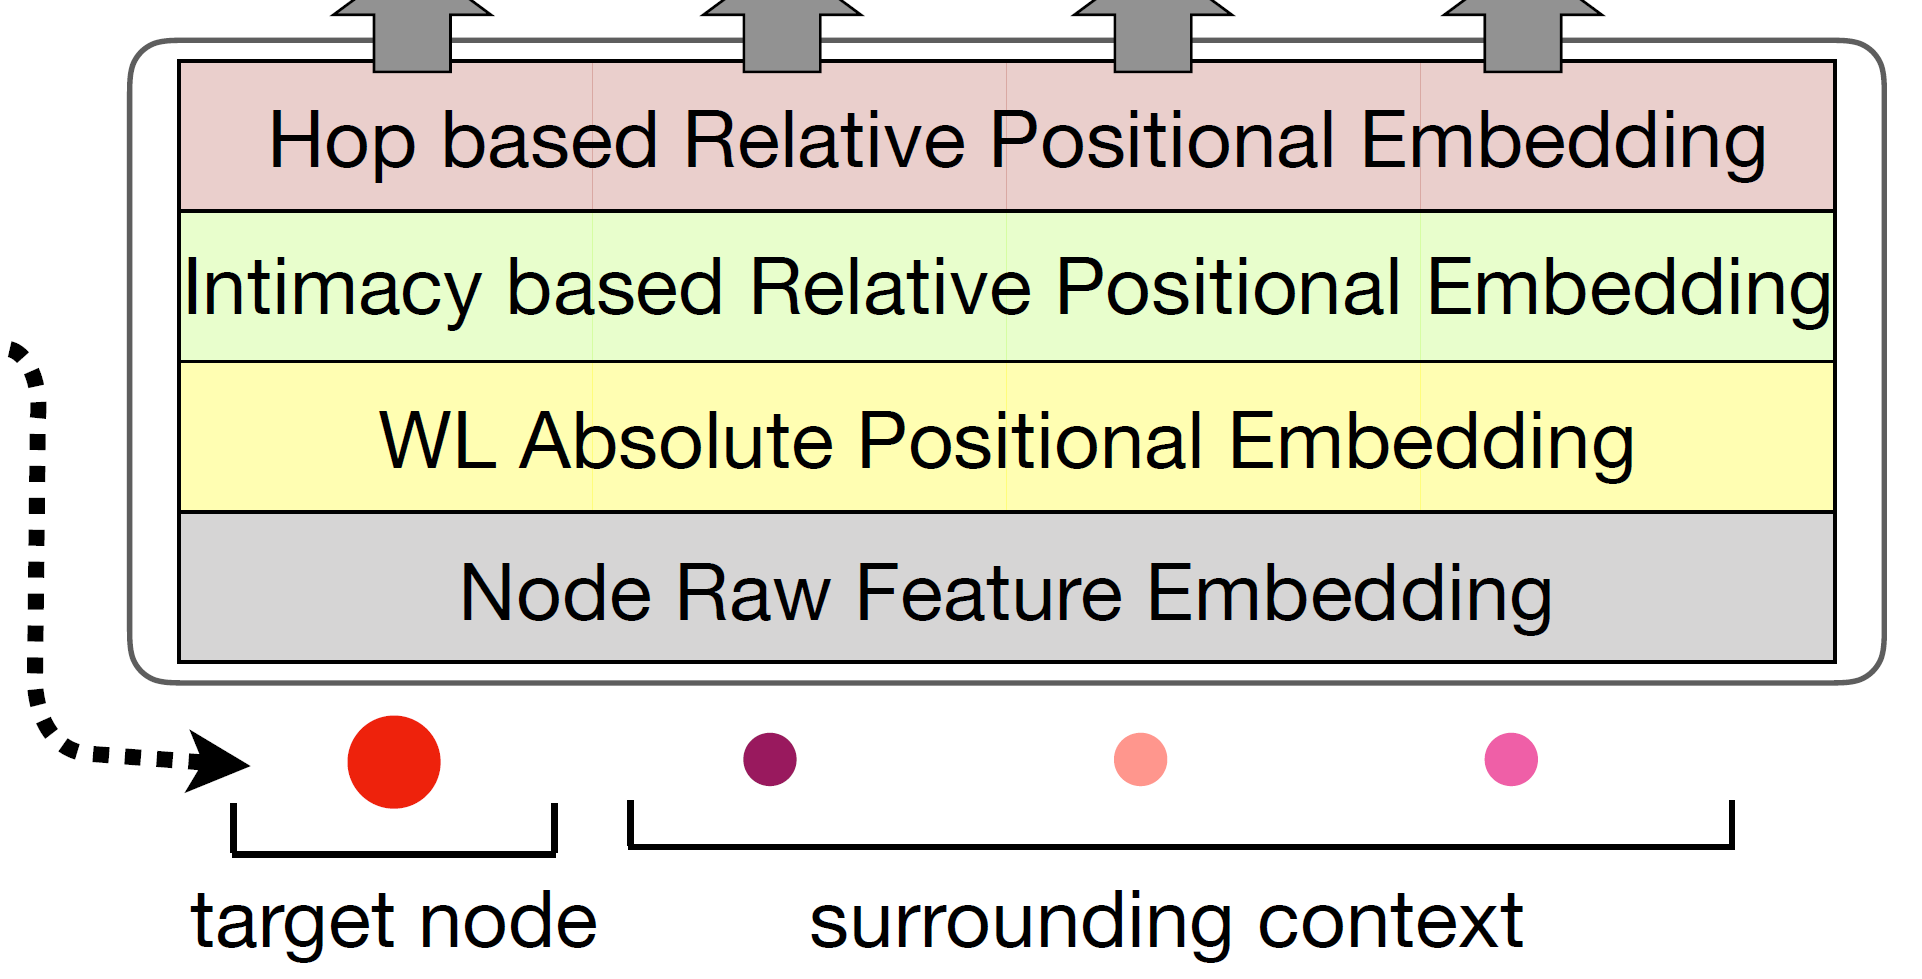
\includegraphics[width=0.7\textwidth]{figures/embeddings}
		\end{figure}
		\begin{itemize}
			\item Raw Feature Vector Embedding
			\item Weisfeiler Lehman Absolute Role Embedding
			\item Intimacy based Relative Positional Embedding
			\item Hop based Relative Distance Embedding 
		\end{itemize}
	}

	\frame {
		\frametitle{Node input vector embeddings}
		\framesubtitle{Raw feature vector embedding}
		
		In each subgraph $g_i$
		
		$g_i = \{v_i, v_{i,0}, v_{i,1}, v_{i,2}, ..., v_{i,k}\}$
		
		For each node $v_j \in g_i$
		\[
			e^{(x)}_j = Embed(x_j) \in \mathbb{R}^{d_h}
		\] 
		
		Here $Embed(\cdot)$ function can be CNN if $x_j$ denotes images or LSTM/BERT if $x_j$ denotes texts etc...
		
		Use nn.Linear layer to produce feature vector $\mathbb{R}^{d_h}$ for $v_j$
		
	}
	\frame {
		\frametitle{Node input vector embeddings}
		\framesubtitle{Weisfeiler Lehman absolute role embedding}
		
		To "color code" every node according to the following process:
		
		\begin{itemize}
			\item Step 0 Initially assign code "1" to all nodes
			\item Step 1 For every target node $v_i$, concat the color codes of all neighbors (the concatenated string initially will be "1\_1\_1\_1..")
			\item Step 2 Generate hash for the string in Step 1
			\item Step 3 Assign a unique number for every the unique hash, so $v_i$ will have a new "color code"
			\item Repeat from step 1 (until stable or after a number of iterations)
		\end{itemize}
	
		Use set of $(k+1)$ color codes and nn.Embedding to produce feature vector $\mathbb{R}^{d_h}$ for $v_j$
		
	}
	\frame {
		\frametitle{Node input vector embeddings}
		\framesubtitle{Intimacy based relative positional embedding}
		
		Use $k$ entries in $sorted(S(j,:))$ and nn.Embedding to produce feature vector $\mathbb{R}^{d_h}$ for $v_j$
		
		But in code, the intimacy score vector is [0, 1,...,k], not the real score.
	}

	\frame {
		\frametitle{Node input vector embeddings}
		\framesubtitle{Hop based relative distance embedding}
		
		In each subgraph $g_i$
		
		$g_i = \{v_i, v_{i,0}, v_{i,1}, v_{i,2}, ..., v_{i,k}\}$
		
		Construct a hop-list $[0, H(v_{i,0}), H(v_{i,1}), H(v_{i,2}), ..., H(v_{i,k})]$
		
		For e.g. $[0, 1, 1, 2, ..., 3]$
		
		Feed into a nn.Embedding to produce feature vector $\mathbb{R}^{d_h}$ for $v_j$ 
		
	}

	\frame {
		\frametitle{Embeddings aggregation}
		In each subgraph $g_i$
		
		$g_i = \{v_i, v_{i,0}, v_{i,1}, v_{i,2}, ..., v_{i,k}\}$
		
		For $v_j$ $\in$ $g_i$
		
		$h^{(0)}_j = sum(e^{x}_j, e^{r}_j, e^{p}_j, e^{d}_j) \in \mathbb{R}^{d_h} $ 
		
		Organize all vectors into a matrix
		
		$H^{(0)} = [h^{(0)}_i, h^{(0)}_{i,0}, h^{(0)}_{i,1}, h^{(0)}_{i,2}, ..., h^{(0)}_{i,k}]^T \in \mathbb{R}^{(k+1) \times d_h} $ 		
	}

	\frame{
		\frametitle{Graph Transformer based encoder}
		
		\begin{figure}
			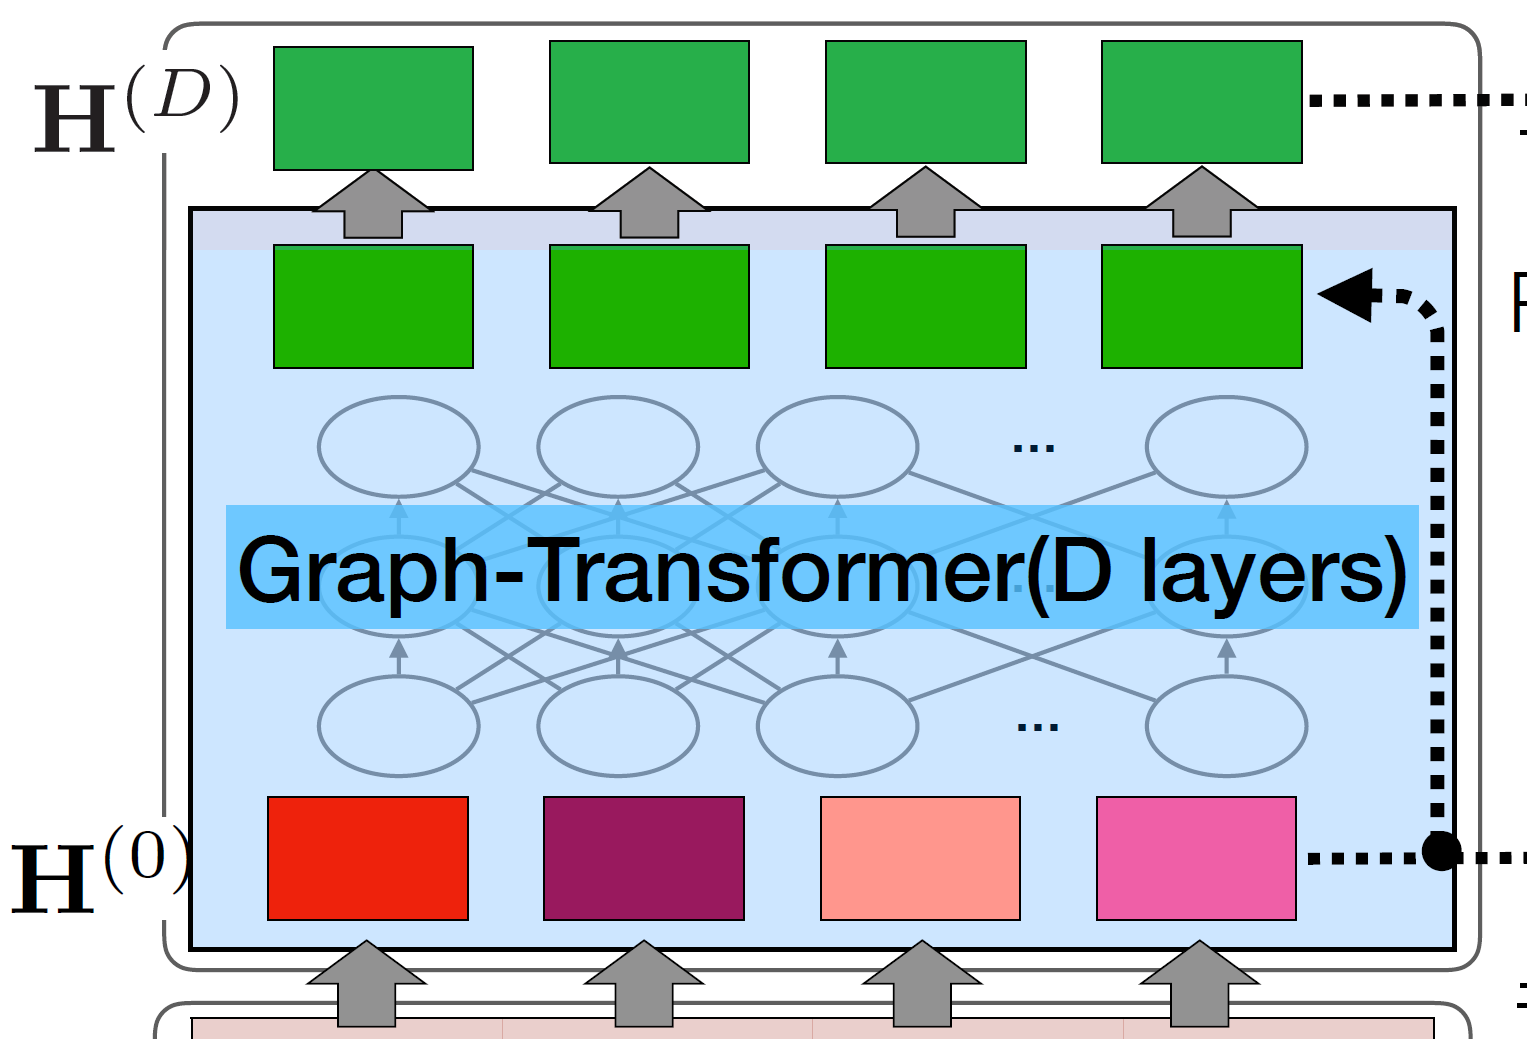
\includegraphics[width=0.7\textwidth]{figures/encoder}
		\end{figure}
	
		
	}

	\frame{
		\frametitle{GRAPH-BERT learning}
		
		\begin{figure}
			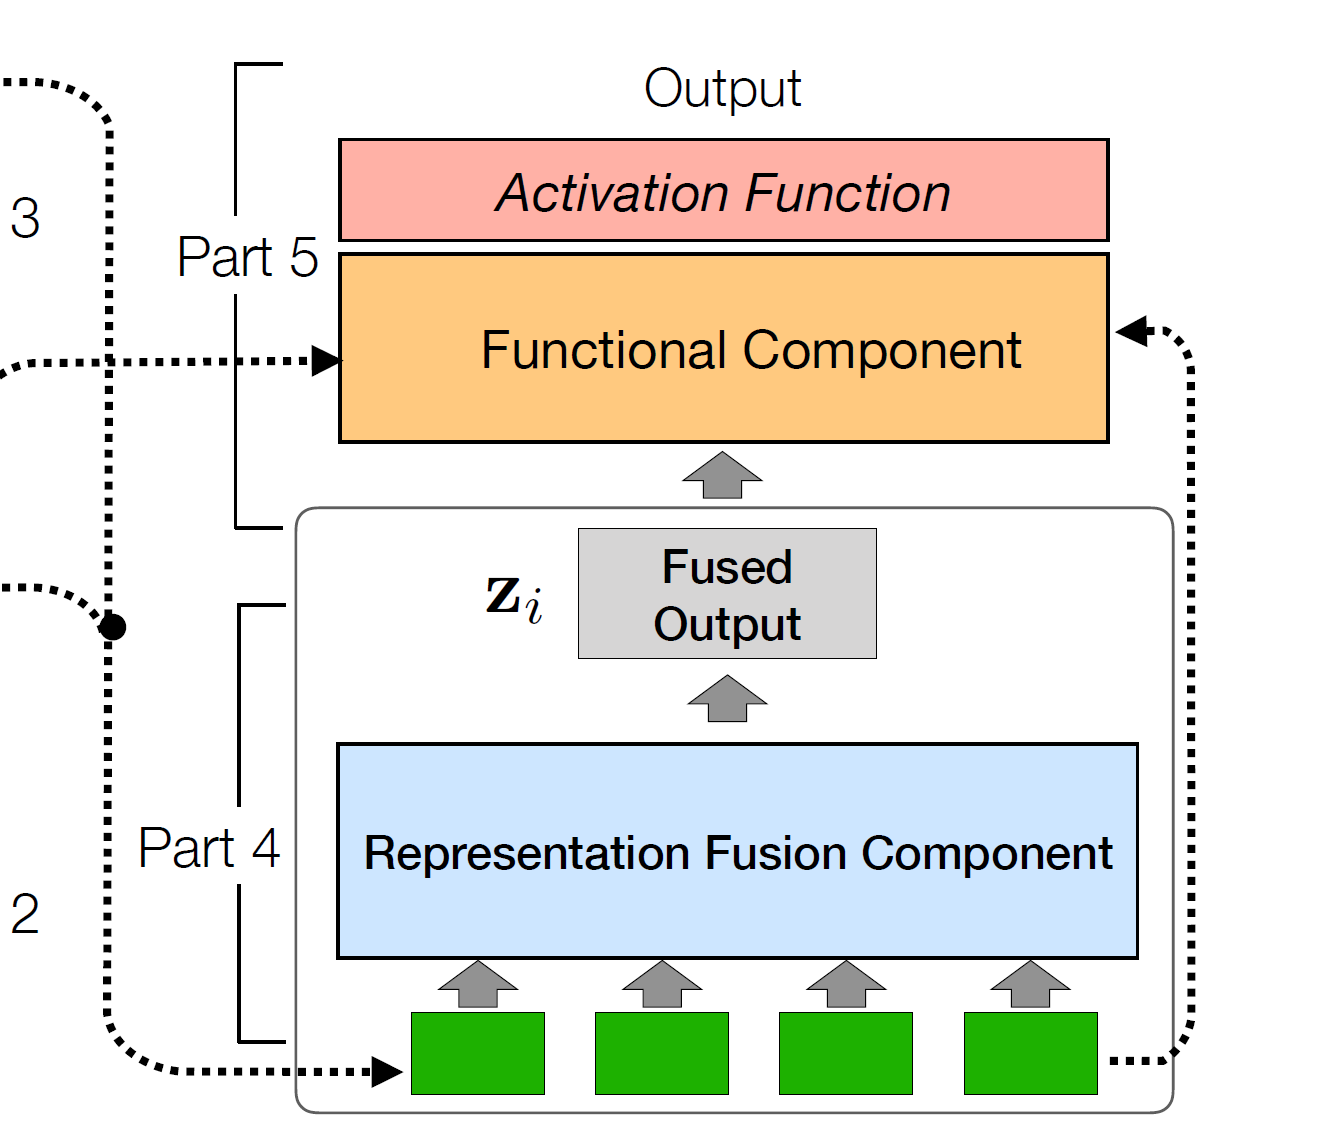
\includegraphics[width=0.45\textwidth]{figures/pretrain}
		\end{figure}
	
		$H^{(D)} \in \mathbb{R}^{(k+1) \times d_h} $ 	
		
		Fusion: $z_i \in \mathbb{R}^{d_h} $ (average out $H^{(D)}$)
		
		FC: nn.Linear(in\_features=$d_h$, out\_features=$x\_size$)
		
		Activation: tanh
	}

	\frame{
		\frametitle{GRAPH-BERT learning}
		\framesubtitle{Pretraining}
		
		Pretrained on 2 tasks
		\begin{itemize}
			\item Node classification
			
			Pretrain using MSE loss on $x_i$ and $\hat{x}_i$
			\[
			l_1 = MSE\_Loss(x_i, \hat{x}_i)
			\]
			
			\item Graph clustering
			
			For any two nodes $v_i$ and $v_j$, compute cosine similarity
			
			\[
				\hat{s}_{i,j} = \frac{z^T_iz_j}{\|{z_i}\|\|{z_j}\|}
			\]
			
			Loss function
			
			\[
				l_2 = \frac{1}{|V|^2}\|S-\hat{S}\|^2_F
			\]
			
			But in code, $A$ is used but not $S$
			
			
			
		\end{itemize}	
	}
	
	\frame{
		\frametitle{Discussion}
		
		\begin{itemize}
			\item Pros
				\item Combine multiple node features
				\item Train on local node context
			\item Cons
			\begin{itemize}
				\item Does not use link features
				
			\end{itemize}
		\end{itemize}
	}
	
\end{document}